% Haskell Symposium tutorial submission (acmsmall, lightweight double-blind).
% Remove 'anonymous' and 'review' for the camera-ready version.
\documentclass[acmsmall,screen,review,anonymous]{acmart}
\usepackage{listings}
\usepackage{booktabs}
\usepackage{tabularx}
\usepackage{tikz}
\usetikzlibrary{positioning,arrows.meta}
\settopmatter{printacmref=false}
\setcopyright{none}
\citestyle{acmauthoryear}
\lstset{language=Haskell,basicstyle=\small\ttfamily,
  columns=fullflexible,keepspaces=true,showstringspaces=false,
  commentstyle=\normalfont\ttfamily,breaklines=true,frame=single,
  xleftmargin=0.4em,xrightmargin=0.4em,aboveskip=0.7em,belowskip=0.7em}
\lstdefinestyle{output}{language={},basicstyle=\small\ttfamily,frame=none,
  backgroundcolor=\color{black!6},xleftmargin=0.4em,xrightmargin=0.4em}
\newcommand{\code}[1]{\texttt{#1}}
\newcommand{\snippet}[1]{\par\noindent
  \begin{minipage}{\linewidth}
  \lstinputlisting{build/snippets/#1.hs}
  \end{minipage}\par}
% Listings quoted verbatim from SBV's documentation modules, which use wider lines.
\newcommand{\libsnippet}[1]{\par\noindent
  \begin{minipage}{\linewidth}
  \lstinputlisting[basicstyle=\footnotesize\ttfamily]{build/snippets/#1.hs}
  \end{minipage}\par}
\newcounter{exercise}
\newenvironment{exercise}{\refstepcounter{exercise}\par\medskip\noindent
  \textbf{Exercise~\theexercise.}\ }{\par\medskip}

\title{From Counterexamples to Inductive Proofs}
\subtitle{A Tutorial on SBV}
\author{Levent Erk\"{o}k}
\authorsaddresses{}

\begin{document}
\begin{abstract}
SBV is a Haskell library for reasoning about programs with SMT solvers. This
tutorial is a guided path through it for Haskell programmers with no prior
background in automated reasoning. We begin with one-line theorems and
counterexamples, write specifications that are independent of the code they
check, search for values that satisfy constraints, and program a live solver
session from Haskell. We then define symbolic algebraic datatypes and recursive
functions, and prove properties that no solver establishes on its own by
supplying induction and equational reasoning as ordinary Haskell code. A
detailed proof of Kadane's maximum-segment-sum algorithm shows how to find the
right invariant, and an overview of a verified tautology checker shows how such
proofs scale. Finally, we compile a verified function to C. Along the way we
explain the boundary between Haskell evaluation and symbolic reasoning, which is
the source of most surprises for new users. Every listing is extracted from a
companion program that is checked against the current release.
\end{abstract}

\keywords{Haskell, SMT, symbolic programming, theorem proving, induction, tutorial}
\maketitle

%==============================================================================
\section{Introduction}
\label{sec:introduction}

Haskell programmers already state properties of their code: QuickCheck
properties~\citep{quickcheck} are ordinary functions that return \code{Bool},
and a test campaign searches for inputs that falsify them. SBV~\citep{sbv} lets
the same programmer ask a stronger question. A property over \emph{symbolic}
values is translated to logic and handed to an SMT solver, which either proves it
for every input or produces a concrete counterexample:
\begin{lstlisting}
ghci> prove $ \x -> abs (x :: SInteger) .>= 0
Q.E.D.
ghci> prove $ \x -> abs (x :: SInt8) .>= 0
Falsifiable. Counter-example:
  s0 = -128 :: Int8
\end{lstlisting}
The two properties differ only in a type. Over mathematical integers, absolute
values are nonnegative. Over signed bytes, 128 is not representable, so
\code{abs (-128)} is $-128$. The solver did not test this value by luck: it
searched all 256 inputs symbolically and reported the one that fails.

This tutorial is for Haskell programmers who want to use solvers in that way and
then go further. It assumes familiarity with type classes and monads but no
knowledge of SMT, logic, or theorem proving. Each section introduces one idea and
builds on the previous ones:
\begin{itemize}
\item Sections~\ref{sec:first}--\ref{sec:finding} cover proofs, counterexamples,
  specifications, and searches for values satisfying constraints.
\item Section~\ref{sec:host} explains the boundary between Haskell evaluation and
  symbolic reasoning, which governs how recursion and data structures behave.
\item Sections~\ref{sec:queries}--\ref{sec:datatypes} program a live solver
  session and introduce symbolic algebraic datatypes.
\item Sections~\ref{sec:induction}--\ref{sec:tautology} prove properties of
  recursive functions with SBV's theorem-proving layer, TP, ending with a detailed
  proof of Kadane's algorithm and an overview of a verified tautology checker.
\item Section~\ref{sec:codegen} compiles a verified function to C, and
  Section~\ref{sec:hood} explains enough of the implementation to make SBV's
  behavior predictable.
\end{itemize}
Section~\ref{sec:pitfalls} collects the pitfalls in one place, and
Section~\ref{sec:related} relates SBV to other tools.

\paragraph{Following along.}
SBV is on Hackage; add \code{sbv} to a project's dependencies and make an SMT
solver available on the \code{PATH}. Z3~\citep{z3} is the default. A few examples
below use CVC5, and SBV also supports Yices, Bitwuzla, Boolector, MathSAT, ABC,
OpenSMT, and dReal. Most examples need only \code{import Data.SBV}; the solver
programming interface is in \code{Data.SBV.Control}, list operations in
\code{Data.SBV.List}, and the proof layer in \code{Data.SBV.TP}. The supplementary
material contains a single program from which every listing in this paper is
extracted. It runs each example, checks its result independently where that is
possible, and also contains solutions to the exercises.

%==============================================================================
\section{First Proofs and Counterexamples}
\label{sec:first}

\subsection{Symbolic values and their types}

SBV's central type is \code{SBV a}, a symbolic value whose concrete counterpart
has type \code{a}. Abbreviations name the common cases: \code{SBool},
\code{SInteger} (unbounded integers), \code{SWord8} through \code{SWord64} and
\code{SInt8} through \code{SInt64} (bit-vectors with wrap-around arithmetic),
\code{SReal} (exact real numbers), \code{SFloat} and \code{SDouble} (IEEE-754),
\code{SString}, and \code{SList a}. There are also arrays, sets, tuples,
\code{Maybe}, \code{Either}, and user-defined algebraic datatypes.

These types are not interchangeable encodings of one numeric type; each is a
different mathematical problem. The introduction showed that the choice between
\code{SInteger} and \code{SInt8} changes a theorem into a false statement.
Floating point has its own surprises:
\begin{lstlisting}
ghci> prove $ \(x :: SFloat) -> x .== x
Falsifiable. Counter-example:
  s0 = NaN :: Float
\end{lstlisting}
Equality in IEEE-754 is not reflexive, and the solver knows it. Choosing a
symbolic type is choosing the semantics the solver will use, so it deserves the
same care as choosing a type for a production program.

\subsection{Operators with a dot}

Arithmetic on symbolic values uses the ordinary \code{Num} class, so \code{x + 1}
and \code{2 * y} work as expected. Comparisons cannot reuse \code{Eq} and
\code{Ord}: their methods return a Haskell \code{Bool}, which must be known when
Haskell evaluates it, while the result of comparing symbolic values may be
unknown. SBV therefore provides \code{.==}, \code{./=}, \code{.<}, \code{.<=},
\code{.>}, and \code{.>=}, which return \code{SBool}. Boolean connectives are
\code{.\&\&}, \code{.||}, \code{sNot}, and implication \code{.=>}.

For the same reason, Haskell's \code{if-then-else} cannot branch on an
\code{SBool}. The function \code{ite :: Mergeable a => SBool -> a -> a -> a}
builds a symbolic choice that the solver resolves. This distinction between
\emph{Haskell control} and \emph{symbolic control} recurs throughout the
tutorial. When all arguments are known, symbolic operations simply compute:
\code{ite (3 .> 2) 10 20} evaluates to the literal \code{10} without involving a
solver.

\subsection{What \texttt{prove} does}

Calling \code{prove} on a function of symbolic arguments creates a fresh
unknown for each argument, evaluates the function to obtain a symbolic formula
$P(\vec{x})$, and asks the solver whether $\neg P(\vec{x})$ is satisfiable. If it
is not, $P$ holds for every input and SBV prints \code{Q.E.D.} If it is, the
satisfying assignment is a counterexample. A third outcome is possible: for
undecidable or very hard problems, the solver may give up or time out. SBV reports
this as an unknown result, which is neither a proof nor a refutation.

Unknowns can also be created by name inside the \code{Symbolic} monad, which
gives readable counterexamples and allows assumptions:
\begin{lstlisting}
prove $ do x <- sInteger "x"
           y <- sInteger "y"
           constrain $ x .> 0 .&& y .> 0
           pure $ x * y .> 0
\end{lstlisting}
Here \code{constrain} restricts attention to inputs that satisfy the assumption.
A contradictory assumption makes every property provable, so assumptions should
be kept as weak as the property permits.

Table~\ref{tab:interfaces} lists the main ways of using a symbolic model. The
rest of the tutorial visits each of them.

\begin{table}[t]
\caption{Entry points into SBV. All of them consume the same symbolic programs.}
\label{tab:interfaces}
\begin{tabularx}{\linewidth}{@{}l X X l@{}}
\toprule
Interface & You supply & You get back & Section\\
\midrule
\code{prove} & A property & Proof, counterexample, or unknown & \ref{sec:first}--\ref{sec:specs}\\
\code{sat}, \code{allSat} & Constraints on unknowns & One or all satisfying models & \ref{sec:finding}\\
\code{optimize} & Constraints and objectives & An optimal model & \ref{sec:finding}\\
\code{query} & A Haskell program driving the solver & Whatever the program computes & \ref{sec:queries}\\
TP & Lemmas, induction, calculations & Checked proofs with dependencies & \ref{sec:induction}--\ref{sec:tautology}\\
\code{compileToC} & A symbolic function & C source code & \ref{sec:codegen}\\
\bottomrule
\end{tabularx}
\end{table}

%==============================================================================
\section{Writing Specifications}
\label{sec:specs}

A proof is only as good as the property it proves. The most useful properties
compare an implementation with a specification written in a different, simpler
way. Consider addition on unsigned bytes that saturates at 255 instead of
wrapping. An implementation can avoid overflow by testing before it adds, while
the specification can use unbounded integers, where overflow cannot happen:
\snippet{saturating}
The guard \code{x .> 255 - y} cannot overflow, because \code{255 - y} is
representable for every byte \code{y}, and on the other branch \code{x + y} does
not wrap. In the specification, \code{sFromIntegral} converts each byte to an
integer \emph{before} adding. Converting the already wrapped byte sum would
repeat the implementation's arithmetic and could hide its mistakes.
\begin{lstlisting}
ghci> prove satAddSpec
Q.E.D.
\end{lstlisting}
The proof covers all 65,536 input pairs. A tempting alternative implementation
shows why the independent specification matters:
\snippet{wrongAdd}
\begin{lstlisting}[style=output]
ghci> prove $ do { x <- sWord8 "x"; y <- sWord8 "y"; pure (wrongAddSpec x y) }
Falsifiable. Counter-example:
  x = 223 :: Word8
  y = 124 :: Word8
\end{lstlisting}
The sum $223+124=347$ wraps to 91, and no byte is greater than 255, so the
saturation branch is never taken. Had the specification also used byte
arithmetic, it would have agreed with the bug. Your solver may report a different
pair; any pair whose sum exceeds 255 is a valid counterexample, and the companion
checks the reported pair with ordinary Haskell arithmetic.

\begin{exercise}
Write \code{satSub :: SWord8 -> SWord8 -> SWord8}, subtraction that saturates
at 0, together with a specification over \code{SInteger}, and prove that they
agree.
\end{exercise}

%==============================================================================
\section{Finding Values}
\label{sec:finding}

Proving a property asks whether every input satisfies it. The dual question asks
whether \emph{some} input satisfies a constraint, and which one. The function
\code{sat} returns one satisfying model, and \code{allSat} enumerates all of them.
Which bytes are unchanged by squaring?
\snippet{idempotent}
\begin{lstlisting}[style=output]
ghci> idempotentBytes
Solution #1:
  s0 = 1 :: Word8
Solution #2:
  s0 = 0 :: Word8
Found 2 different solutions.
\end{lstlisting}
The answer is a small theorem in disguise: $x(x-1)\equiv 0 \pmod{256}$, and since
$x$ and $x-1$ are coprime, one of them must be divisible by 256.

When some solutions are better than others, \code{optimize} finds the best one.
A workshop makes two products with profits 2 and 3, subject to two resource
limits:
\snippet{production}
\begin{lstlisting}[style=output]
ghci> production
Optimal model:
  x      =  4 :: Integer
  y      =  3 :: Integer
  profit = 17 :: Integer
\end{lstlisting}
With several objectives, the first argument of \code{optimize} selects how to
combine them: lexicographically, independently, or as a Pareto front. Over
\code{SInteger} this is integer linear programming; replacing the types with
\code{SReal} gives linear programming over the rationals.

%==============================================================================
\section{Haskell Structure and Symbolic Structure}
\label{sec:host}

Every SBV program runs in two stages. First, Haskell evaluates the program and
builds a symbolic formula. Second, the solver reasons about that formula. Knowing
which stage handles which part of a program explains most of SBV's behavior.

\subsection{Haskell lists of symbolic values}

A Haskell list \code{[SInteger]} has a spine that Haskell owns and elements that
may be symbolic. Functions such as \code{sum}, \code{map}, and \code{foldr} work
on it unchanged, because they only rearrange the spine and apply \code{Num}
operations to the elements:
\snippet{hostSum}
For any fixed \code{n}, \code{prove (nonNegSum 5)} succeeds immediately. Haskell
unfolds \code{sum} into \code{x1 + x2 + x3 + x4 + x5} before the solver sees
anything; the recursion has disappeared. This style is ideal for fixed-size
problems: circuits, unrolled loops, puzzles on fixed boards. The price is that
the theorem is about lists of length five, not all lists.

\subsection{Symbolic lists and recursive functions}

The type \code{SList Integer} is a list whose length and contents are both
unknown. To state a property of \emph{every} list, we need a function whose
recursion is part of the logic, not something Haskell unfolds. Writing a naive
recursive Haskell function over \code{SList} does not work: whether the list is
empty is unknown, so Haskell would unfold both branches forever.
SBV's \code{smtFunction} solves this problem. It gives the function a name, and
recursive calls become calls to that named function in the logic:
\snippet{sumL}
The \code{sCase} quasi-quoter provides pattern matching on symbolic values. The
definition reads like ordinary Haskell, but SBV translates it to a single
recursive SMT-LIB definition~\citep{smtlib}. Because \code{sumL} is a function
of symbolic values, it still computes on literals: \code{sumL [1,2,3]} evaluates
to \code{6} without a solver. SBV also checks that recursive definitions
terminate; for \code{sumL}, it finds a suitable measure automatically.

Now try the obvious generalization of \code{nonNegSum}:
\begin{lstlisting}
prove $ \xs -> SL.all (.>= 0) xs .=> sumL xs .>= 0
\end{lstlisting}
The property is true, but proving it requires induction on the list, and SMT
solvers do not perform induction. Typically the solver runs until it is stopped
or reports an unknown result. Section~\ref{sec:induction} shows how to supply
the induction ourselves.

The general rule is: \emph{recursion over Haskell structure happens while building
the problem; recursion through \code{smtFunction} becomes part of the problem}.
The former yields bounded but fully automatic results; the latter yields
unbounded results that may need a proof.

%==============================================================================
\section{Programming the Solver}
\label{sec:queries}

The functions \code{prove}, \code{sat}, and \code{optimize} each run a single
solver interaction. Many applications need a conversation: ask, inspect the
answer, and ask a refined question. SBV's \code{query} mode hands control of a
live solver session to a Haskell program. The following function finds the
smallest integer greater than 10 that leaves remainder 3 when divided by 7 and
remainder 4 when divided by 5:
\snippet{descent}
\begin{lstlisting}[style=output]
ghci> smallest
24
\end{lstlisting}
The constraints before \code{query} set up the problem as usual. Inside the
query, \code{checkSat} asks for a model, and \code{getValue} reads the value of
\code{x} in that model. That value is an ordinary \code{Integer}, so Haskell can
branch on it and use it to build the next constraint, \code{x .< literal v},
which asks for a smaller solution. When no smaller solution exists, the last
model found is the minimum. The \code{case} on the solver's answer is Haskell
control; the constraint that it adds is symbolic. Keeping the two apart is what
makes the solver usable as a component of a larger algorithm.

Three properties of this loop are worth noting. First, it terminates only
because the constraints admit a least solution; the same loop over a set
without a minimum would run forever, even though each call to the solver
returns. The termination argument belongs to the client algorithm, not to the
solver. Second, the solver may return the candidates in any order. Our loop
does not depend on that order; it only relies on unsatisfiability at the end.
Third, the loop handles an unknown answer separately: an inconclusive solver
response is not evidence that no smaller value exists.

Queries can do much more: \code{push} and \code{pop} add and retract temporary
assumptions, named constraints allow unsatisfiable cores to be extracted, and new
unknowns can be created in the middle of a session with \code{freshVar}. The last
point is less trivial than it looks: a new variable may have a type, such as a
user-defined datatype, that the solver has not seen yet. SBV tracks the
declarations each new term needs and sends them before the term is used, so
queries compose without regard to the order in which types are first used.

\begin{exercise}
Change \code{smallest} to find the \emph{largest} solution below 100. (The answer
is 94.)
\end{exercise}

%==============================================================================
\section{Symbolic Datatypes}
\label{sec:datatypes}

User-defined algebraic datatypes become symbolic with one line of Template
Haskell. Here is a tiny expression language and its evaluator:
\snippet{expr}
The call \code{mkSymbolic [''Expr]} generates the type \code{SExpr}, symbolic
constructors (\code{sNum}, \code{sAdd}, \code{sMul}), recognizers (\code{isNum},
\code{isAdd}, \code{isMul}), and field accessors such as \code{getMul\_1}. The
evaluator is an \code{smtFunction}, so it is a recursive definition in the
logic, and \code{sCase} matches on an expression whose constructor may be
unknown. The puzzle asks the solver to \emph{synthesize} an expression: a
multiplication whose left argument is not a number, evaluating to 42.
\begin{lstlisting}[style=output]
ghci> puzzle
Satisfiable. Model:
  s0 = Mul (Mul (Num 1) (Num (-1))) (Num (-42)) :: Expr
\end{lstlisting}
The model is an ordinary Haskell value of type \code{Expr}, which we can inspect,
print, or evaluate with a separate Haskell interpreter. The companion does exactly
that to check the answer independently of the solver. Different solver versions
may find different expressions.

The same datatype can be the subject of proofs: a property of \code{eval} over
all expressions is a statement about an unbounded, recursive structure, and will
need induction. That is the topic of the next section.

%==============================================================================
\section{Proofs by Induction}
\label{sec:induction}

SMT solvers decide many theories well, but they do not discover induction
arguments. SBV's TP layer (in \code{Data.SBV.TP}) lets the programmer write the
argument in Haskell and has the solver check each step. The programmer decides
\emph{what} to prove and \emph{how} to break it into steps; the solver decides
whether each step is valid.

\subsection{A first inductive proof}

We return to the property that eluded \code{prove} in Section~\ref{sec:host}:
\snippet{sumNonNeg}
The type \code{Proof (Forall "xs" [Integer] -> SBool)} records the statement of
the theorem: for every integer list \code{xs}, a property holds. The name in
\code{Forall} documents the quantified variable and is used in output and
instantiation. The function \code{induct} applies list induction: SBV checks the
base case (the empty list) automatically and gives the user the inductive step.
In that step, \code{ih} is the induction hypothesis, a proof of the property for
\code{xs}, and the goal is to show it for \code{x .: xs}.

The step is a \emph{calculation}. Its first line lists the assumptions, here the
precondition for the longer list, and \code{|-} starts a chain of expressions
connected by \code{=:}. Each link must be justified by the definitions, the
assumptions, and any hints supplied with \code{??}. The chain ends with
\code{qed}. Running the proof shows each checked step:
\begin{lstlisting}[style=output]
ghci> runTP sumNonNeg
Inductive lemma: sumNonNeg
  Step: Base                  Q.E.D.
  Step: 1                     Q.E.D.
  Step: 2                     Q.E.D.
  Result:                     Q.E.D.
Functions proven terminating: sbv.foldr, sumL
\end{lstlisting}
Step~1 unfolds \code{sumL} once. Step~2 uses the hypothesis: \code{x} is
nonnegative by assumption and so is \code{sumL xs}, so the sum is too. The
\code{Result} line checks that the chain, together with the base case, establishes
the theorem as stated. The last line reports that the recursive functions used,
including the library's \code{foldr} that underlies \code{SL.all}, were checked for
termination.

\subsection{What the solver checks}

A calculation $e_0 = e_1 = \cdots = e_n$ under assumptions $A$, with hints
$H_i$ attached to step $i$, generates one solver query per step:
\[
  A \land H_i \land \neg(e_i = e_{i+1}) \quad\text{must be unsatisfiable.}
\]
Each query is small and local. This is why calculations work: the solver never
has to find the overall argument, only to confirm that consecutive expressions
are equal. If a step fails, SBV reports which one, which turns proof debugging
into a question about one equation. A step that is too large can be split by
adding intermediate expressions; a step that fails although it is true usually
needs a hint.

\subsection{Generalizing the statement}

Reversing a list with an accumulator is a standard optimization:
\snippet{revAcc}
We expect \code{revAcc [] xs} to equal \code{SL.reverse xs}. The direct attempt
is instructive:
\snippet{revWeak}
\begin{lstlisting}[style=output]
ghci> runTP revWeak
Inductive lemma: revWeak
  Step: Base                Q.E.D.
  Step: 1                   Q.E.D.
  Step: 2
*** Failed to prove revWeak.2.
\end{lstlisting}
Step~2 tries to use the induction hypothesis, but the hypothesis is about
\code{revAcc [] xs}, while the expression contains \code{revAcc [x] xs}. After
one step of recursion, the accumulator is no longer empty, and the hypothesis says
nothing about it. (We ran this with a five-second timeout; without one, the
solver searches until it is interrupted.)

The fix is the oldest trick in inductive proofs: prove a more general statement.
The theorem must describe \code{revAcc} for \emph{every} accumulator, so that the
hypothesis can be used at whatever accumulator the recursion produces:
\snippet{revAccCorrect}
Here \code{acc} is universally quantified, and the induction hypothesis
\code{ih} holds for all accumulators. When it is supplied as a hint, the solver
instantiates it with \code{x .: acc}. The remaining steps use ordinary laws of
\code{++} and \code{reverse}, which the solver knows. The original statement is
the special case \code{acc = []}, which a one-line \code{lemma} can derive.

\begin{exercise}
Prove that \code{SL.length (revAcc acc xs) .== SL.length xs + SL.length acc}.
Does the statement need to be generalized, and why?
\end{exercise}

%==============================================================================
\section{Case Study: Kadane's Algorithm}
\label{sec:kadane}

The maximum segment sum problem asks for the largest sum of a contiguous segment
of a list, where the empty segment has sum 0. For
\code{[1, -2, 3, 4, -1, 2]}, the answer is 8, from \code{[3, 4, -1, 2]}.
Kadane's algorithm~\citep{bentley} solves it in a single left-to-right pass.
Its correctness is not obvious, which makes it a good example of finding and
proving an invariant.

\subsection{Specification}

We specify the problem by its most direct recursive reading:
\snippet{mss}
\code{mssBegin xs} is the best sum of a segment that starts at the beginning of
\code{xs}: either the empty segment (0), just the head, or the head followed by
the best segment starting at the tail. \code{mss xs} is the best of
\code{mssBegin xs} and the best segment of the tail. These definitions are clearly
correct and clearly inefficient: they take quadratic time. Since they are
symbolic functions, they also run on literal lists, which is a convenient way to
test a specification before reasoning about it:
\code{mss [1, -2, 3, 4, -1, 2]} evaluates to \code{8}.

\subsection{Implementation}

Kadane's algorithm maintains two accumulators while it scans the list:
\code{meh}, the maximum sum of a segment ending at the current position, and
\code{msf}, the maximum found so far:
\snippet{kadane}
At each element \code{h}, the best segment ending here either extends the best
segment ending at the previous position or is empty, so the new \code{meh} is
\code{0 `smax` (h + meh)}. The best so far is updated if that value is larger.

\subsection{Finding the invariant}

As with reversal, the theorem we want, \code{kadane xs .== mss xs}, concerns the
initial accumulators \code{0} and \code{0}. An inductive proof will reach
\code{kadaneHelper} with other accumulator values, so we must describe what
\code{kadaneHelper xs meh msf} computes for \emph{any} sensible \code{meh} and
\code{msf}.

Think of the list as split into a prefix that has been processed and a suffix
\code{xs} that has not. The best segment of the whole list lies in one of three
places:
\begin{enumerate}
\item entirely within the prefix: its sum is \code{msf};
\item entirely within the suffix: its sum is \code{mss xs};
\item across the boundary: it is a segment ending at the boundary, whose best sum
  is \code{meh}, followed by a segment starting at the boundary, whose best sum is
  \code{mssBegin xs}.
\end{enumerate}
So the invariant is
\[
  \mathit{kadaneHelper}(xs, \mathit{meh}, \mathit{msf})
  = \max\bigl(\mathit{msf},\ \mathit{mss}(xs),\ \mathit{meh} + \mathit{mssBegin}(xs)\bigr),
\]
under the preconditions that make the accumulators meaningful:
$\mathit{meh} \geq 0$ (the empty segment is always available) and
$\mathit{msf} \geq \mathit{meh}$ (the best segment so far is at least as good as
the best one ending here). Without the preconditions the statement is false: for
an empty \code{xs}, the right side would include $\mathit{meh}$ even when it
exceeds $\mathit{msf}$.

\subsection{The proof}

Once the invariant is written down, the proof is short:
\snippet{kadaneCorrect}
The inductive step unfolds \code{kadaneHelper} once and applies the hypothesis
at the new accumulators. Here the hint is more specific than in the earlier
proofs: \code{ih `at` (Inst @"meh" meh', Inst @"msf" msf')} instantiates the
quantified accumulators explicitly. The solver could search for the
instantiation, but stating it makes the step easier and documents the argument.
The remaining equality between the instantiated hypothesis and the invariant
for \code{a .: as} is arithmetic over \code{smax}, which the solver checks
without further help, using the definitions of \code{mss} and \code{mssBegin}.
The preconditions are needed to instantiate the hypothesis: the new accumulators
satisfy them because \code{meh'} is a maximum with 0 and \code{msf'} is a
maximum with \code{meh'}.

The main theorem then follows by a calculation without induction. With both
accumulators 0, the invariant gives
$\max(0, \mathit{mss}(xs), \mathit{mssBegin}(xs))$, and the solver discharges the
last two steps: \code{mss} is nonnegative and at least \code{mssBegin} by its
definition.
\begin{lstlisting}[style=output]
ghci> runTP kadaneCorrect
Inductive lemma: kadaneInvariant
  Step: Base                        Q.E.D.
  Step: 1                           Q.E.D.
  Step: 2                           Q.E.D.
  Result:                           Q.E.D.
Lemma: kadaneCorrect
  Step: 1                           Q.E.D.
  Step: 2                           Q.E.D.
  Step: 3                           Q.E.D.
  Step: 4                           Q.E.D.
  Result:                           Q.E.D.
Functions proven terminating: kadaneHelper, mss, mssBegin
\end{lstlisting}
The whole proof takes about a tenth of a second with Z3.

\subsection{Lessons}

The effort in this proof went into one place: the invariant. Once we had
explained \emph{why} the algorithm works, as the three-way case analysis on where
the best segment lies, the mechanical checking was immediate. This division of
labor is typical of TP. The solver handles unfolding definitions, arithmetic,
and case analysis on \code{smax}; the human supplies generalizations and
intermediate statements. When a proof gets stuck, the useful question is
rarely ``which tactic is missing?'' and usually ``what is the statement that
explains this step?''

%==============================================================================
\section{Case Study Overview: A Verified Tautology Checker}
\label{sec:tautology}

Larger developments are built from the same ingredients. SBV's documentation
includes a verified tautology checker for propositional formulas in
if-then-else form, after a classic development by \citet{boyermoore} that was
later formalized in Imandra~\citep{imandraTautology}. We sketch its structure
rather than its proofs; the full development is in the module
\code{Documentation.\allowbreak SBV.\allowbreak Examples.\allowbreak TP.\allowbreak TautologyChecker}. The listings in this
section are quoted from that module.

\paragraph{Formulas and normalization.}
A formula is a constant, a variable, or a conditional:
\libsnippet{tautFormula}
The checker first normalizes a formula so that no conditional appears in the
condition position of another conditional, by repeatedly rewriting
\code{If (If p q r) l r'} to \code{If p (If q l r') (If r l r')}. Abbreviated
slightly, the definition is:
\begin{lstlisting}
normalize :: SFormula -> SFormula
normalize = smtFunctionWithMeasure "normalize"
    ( \f -> tuple (ifComplexity f, ifDepth f)
    , [measureLemma ifDepthNonNeg, measureLemma ifComplexityPos, ...] )
  $ \f -> [sCase| f of
             If (If p q r) l r' -> normalize (sIf p (sIf q l r') (sIf r l r'))
             If c l r           -> sIf c (normalize l) (normalize r)
             _                  -> f
          |]
\end{lstlisting}
This function is the first new ingredient. Its termination is not structural:
the rewrite in the first branch produces a \emph{larger} formula. Instead of
letting SBV guess a measure, the definition supplies one through
\code{smtFunctionWithMeasure}: a pair
ordered lexicographically: a complexity measure that the rewrite does not
increase, and the depth of conditionals in condition position, which it
decreases. Each \code{measureLemma} is a proved lemma that SBV uses when checking
the measure; for example, that the complexity of a formula is positive.

\paragraph{Checking.}
On a normalized formula, the checker walks down the conditionals, recording an
assumed value for each variable the first time it is tested. When it meets a
variable that was already assigned, it follows the corresponding branch;
otherwise it checks both branches, once under each assumption. The function
\code{isTautology f} normalizes \code{f} and runs this walk with no assumptions.

\paragraph{The theorems.}
Soundness says that a formula accepted by the checker evaluates to true under
every assignment:
\libsnippet{tautSoundness}
Completeness says that if the checker rejects a formula, a companion function
\code{falsify} produces an assignment under which the formula is false:
\libsnippet{tautCompleteness}
Both top-level proofs are short because the work is in their lemmas. The
development contains 21 TP lemmas. Several prove properties of variable lookup
when assignments are extended; others establish that normalization produces a
normal formula and preserves meaning. The central inductive lemmas, such as
\code{tautologyImpliesEval}, use \emph{strong induction} via \code{sInduct}:
the hypothesis is available for every formula with a smaller measure, not only
for immediate subformulas, which matches the shape of the recursion in
\code{isTautology'}. The lemmas use \code{recall} to reuse previously proved
results and, in a few places, select CVC5 instead of Z3 for steps where it
performs better. Soundness and completeness each check in one to two seconds.

\paragraph{What to take away.}
The development reuses every technique from the earlier sections at larger
scale. Generalization appears again: the central lemma \code{tautologyImpliesEval} is
stated for arbitrary variable assignments, not only for the empty list of
assumptions with which \code{isTautology} starts. New
techniques are explicit termination measures and strong induction. The structure
of the proof follows the structure of the program: one group of lemmas per
auxiliary function, and top-level theorems assembled from them by short
calculations. SBV's documentation contains about forty further TP developments,
including sorting algorithms, a semantics-preserving constant folder, and a
compiler from expressions to a stack machine.

%==============================================================================
\section{From Verified Code to C}
\label{sec:codegen}

The symbolic programs we have written can also be compiled. SBV translates a
symbolic function to C code that runs without a solver. For the saturating adder
of Section~\ref{sec:specs}:
\snippet{codegen}
This produces \code{sat\_add.c} and a matching header. Because the C code is
generated from the same \code{satAdd} that we proved correct, there is no manual
rewrite in which the two could drift apart. Bit-vector operations are generated
with explicit widths and signedness, so the code does not depend on C's integer
promotion rules or on undefined signed overflow.

Code generation is not a verified compiler, and it is worth being precise about
what is known. The proof establishes a property of the \emph{symbolic} function.
The C program is a separate artifact, produced by a translation that must
implement each operation faithfully. For a function with a small input domain we
can close the gap by testing: the companion compiles the generated adder with
undefined-behavior sanitization and compares it on all 65,536 inputs with an
independent oracle written directly in C. The proof and the exhaustive test
make different claims, about the model and about the compiled code, and together
they give confidence in both.

Not all of SBV's vocabulary is executable. Quantifiers and uninterpreted sorts,
for example, have no operational meaning, and the code generator rejects programs
that use them rather than approximating them. Uninterpreted functions become calls
to C functions that the user provides, which then join the trusted code.

%==============================================================================
\section{Under the Hood}
\label{sec:hood}

This section explains enough of SBV's implementation to make its behavior
predictable. Figure~\ref{fig:architecture} shows the overall flow.

\begin{figure}[t]
\centering
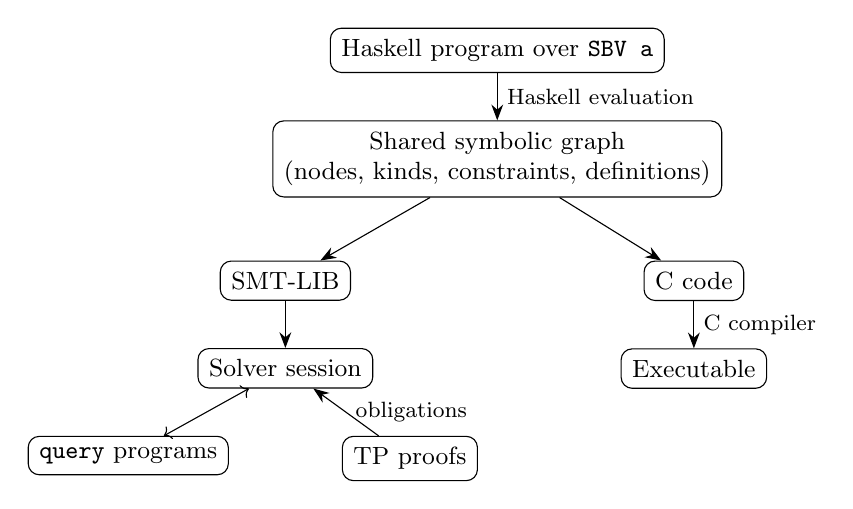
\begin{tikzpicture}[node distance=6mm and 8mm,
    box/.style={draw,rounded corners,align=center,inner sep=4pt,font=\small},
    arr/.style={-{Stealth[length=2mm]}}]
\node[box] (hs) {Haskell program over \code{SBV a}};
\node[box,below=of hs] (graph) {Shared symbolic graph\\(nodes, kinds, constraints, definitions)};
\node[box,below left=8mm and -10mm of graph] (smt) {SMT-LIB};
\node[box,below right=8mm and -10mm of graph] (c) {C code};
\node[box,below=of smt] (solver) {Solver session};
\node[box,below left=6mm and -4mm of solver] (q) {\code{query} programs};
\node[box,below right=6mm and -4mm of solver] (tp) {TP proofs};
\node[box,below=of c] (exe) {Executable};
\draw[arr] (hs) -- node[right,font=\footnotesize]{Haskell evaluation} (graph);
\draw[arr] (graph) -- (smt);
\draw[arr] (graph) -- (c);
\draw[arr] (smt) -- (solver);
\draw[arr] (c) -- node[right,font=\footnotesize]{C compiler} (exe);
\draw[arr,<->] (q) -- (solver);
\draw[arr] (tp) -- node[right,font=\footnotesize]{obligations} (solver);
\end{tikzpicture}
\caption{Haskell evaluation builds a shared graph, which is translated to SMT-LIB
for the solver or to C for execution. Queries and proofs drive the solver.}
\Description{A Haskell program over symbolic values is evaluated into a shared
symbolic graph. The graph is translated either to SMT-LIB, feeding a solver
session that query programs and TP proofs interact with, or to C code.}
\label{fig:architecture}
\end{figure}

\paragraph{Symbolic values are deferred graph nodes.}
Internally, a value of type \code{SBV a} is either a concrete constant or a
deferred computation that, given the state of the current symbolic run, adds a
node to a graph and returns its identifier:
\begin{lstlisting}
newtype SBV a = SBV SVal
data SVal     = SVal Kind (Either CV (Cached SV))
newtype Cached a = Cached (State -> IO a)
\end{lstlisting}
This representation lets \code{x + y} have the pure type
\code{SWord8 -> SWord8 -> SWord8} while still allocating graph nodes. Operations
on constants are folded immediately, which is why \code{satAdd 250 10} evaluates
to \code{255} without a solver. The run-time \code{Kind} records the logical sort,
so simplifications can respect it: rewriting \code{x .== x} to true is valid for
integers but not for floats.

\paragraph{Sharing comes in two forms.}
A generator that combines a term with itself, such as
\code{iterate (\textbackslash{}t -> t + t) x !! 30}, describes a term that is
exponentially large as a tree but linear as a graph. SBV preserves this sharing
in two ways. It memoizes each deferred computation, using stable names in the
style of observable sharing~\citep{sharing}, so that forcing the same Haskell
value twice yields the same node. It also interns nodes, so that separately
constructed applications of the same operator to the same arguments reuse a node.
Neither mechanism identifies arbitrary mathematically equal expressions.

\paragraph{Nodes belong to a run.}
A graph node is meaningful only in the run that created it. Two values of type
\code{SInteger} from different calls to \code{prove} cannot be combined, even
though their types agree, and SBV checks for common mistakes of this kind. To
carry a result from one run to another, extract a concrete value from a model
and turn it back into a literal, as the query in Section~\ref{sec:queries} does
with \code{literal v}.

\paragraph{Queries synchronize dependencies.}
When a query creates a new term, SBV records the declarations it requires: sorts
for datatypes (including those nested inside lists, tuples, or other datatypes),
uninterpreted constants, and definitions of \code{smtFunction}s it calls. Before
the term is used, any of these that the solver has not seen are sent. This is why
the datatype example in Section~\ref{sec:datatypes} works even when the datatype
first appears inside a query.

%==============================================================================
\section{Pitfalls and What to Trust}
\label{sec:pitfalls}

\paragraph{Common pitfalls.}
\begin{itemize}
\item \emph{Wrong domain.} A property proved over \code{SInteger} says nothing
  about \code{SInt32}, and vice versa. Choose the type that matches the code you
  care about.
\item \emph{Specification repeats the implementation.} Write specifications in a
  different style or a wider domain (Section~\ref{sec:specs}).
\item \emph{Haskell \code{if} or recursion on symbolic data.} Use \code{ite} and
  \code{sCase} for symbolic choices, and \code{smtFunction} for recursion over
  symbolic structure (Section~\ref{sec:host}).
\item \emph{Contradictory assumptions.} If \code{constrain}ed assumptions are
  unsatisfiable, everything is provable. A quick \code{sat} on the assumptions
  alone detects this.
\item \emph{Treating unknown as an answer.} A timeout or unknown result is
  neither a proof nor a counterexample.
\item \emph{Too specific an induction statement.} If a proof step involving the
  induction hypothesis fails, the statement probably needs generalizing
  (Sections~\ref{sec:induction} and~\ref{sec:kadane}).
\item \emph{Mixing runs.} Symbolic values do not survive the run that created
  them; move concrete values instead (Section~\ref{sec:hood}).
\end{itemize}

\paragraph{What a proof rests on.}
A Q.E.D. from SBV depends on the correctness of SBV's translation to SMT-LIB, the
solver, and, for TP, the generation of proof obligations. TP proofs also depend on
any axioms the user introduces and on any functions whose termination checks
were explicitly bypassed. SBV tracks these dependencies: a proof that rests on an
axiom, or on an unfinished step marked with \code{sorry}, is reported as
\code{Modulo} the offending lemmas rather than as \code{Proven}. TP does not replay solver certificates in an independent proof
kernel, so its guarantees are those of the underlying solver. Properties of
symbolic lists are properties of finite lists: unlike Haskell lists, symbolic
lists contain no bottoms and no infinite values. For generated C, the C compiler
and the code generator join the trusted base, which is why
Section~\ref{sec:codegen} validates the generated code separately.

%==============================================================================
\section{Related Tools and Further Reading}
\label{sec:related}

QuickCheck~\citep{quickcheck} and SBV ask similar questions with different
evidence: a passing test campaign samples the input space, while an
unsatisfiability result covers it. The two combine well, and SBV's own test
suite compares concrete evaluation with solver results using QuickCheck.

Several systems embed solver-aided programming in a host language.
Rosette~\citep{rosette} provides a symbolic virtual machine for Racket that
lifts ordinary host constructs to symbolic values. Grisette~\citep{grisette} is
a Haskell library for symbolic compilation that focuses on efficient symbolic
evaluation of programs with state merging. Smten~\citep{smten} translated
high-level Haskell-like symbolic computations into SMT queries. The what4
library~\citep{what4} offers a typed Haskell interface to many solvers and is
used inside verification tools. SBV makes the boundary between Haskell and
symbolic control explicit through its types and operators, and adds the TP proof
layer and C generation on the same representation.

For proofs about Haskell programs, Liquid Haskell~\citep{liquidhaskell} checks
refinement types with an SMT solver, and refinement reflection~\citep{reflection}
extends it to equational proofs about user-defined functions. There, specifications
are refinement types on the program itself and proofs are Haskell terms checked
against them; SBV's TP proofs are instead separate Haskell programs about
symbolic models. Dafny~\citep{dafny} shows
how far the combination of user-supplied invariants and automatic
verification-condition discharge can go in a dedicated language.

The SBV distribution contains a large collection of documented examples under
\code{Documentation.\allowbreak SBV.\allowbreak Examples}, covering puzzles, cryptography, code
generation, optimization, and theorem proving. The TP examples mentioned in
Section~\ref{sec:tautology} are a good next step after this tutorial.

%==============================================================================
\section{Conclusion}

SBV lets a Haskell programmer move gradually from checking a single arithmetic
fact to proving properties of recursive algorithms, using one vocabulary of
symbolic values throughout. The skills that matter change along the way:
choosing the semantic domain, writing an independent specification, separating
Haskell control from symbolic control, and, for inductive proofs, finding a
statement general enough to prove. The solver handles the rest. We hope the
examples here, all of which run, encourage readers to bring a solver into their
own Haskell programs.

\bibliographystyle{ACM-Reference-Format}
\bibliography{references}
\end{document}
